
\documentclass{beamer}
\usetheme{BauhausNeuralFEM} 
\usepackage{amssymb}

\title[Strong and Weak Forms]{From FEM to Neural Operators: Scientific Machine Learning for Computational Mechanics\\[0.4cm]}
\subtitle{From Strong to Weak Form:\\The Basis of the Finite Element Method}
\author{Dr-Ing Jorge Alberto L\'{o}pez Zerme\~{n}o}
\date{}

\graphicspath {{Figures/}}

\begin{document}

%====================================================
{
	\usebackgroundtemplate{
		\begin{tikzpicture}[remember picture,overlay]
			\node[opacity=0.25,inner sep=0pt] at (current page.center)
			{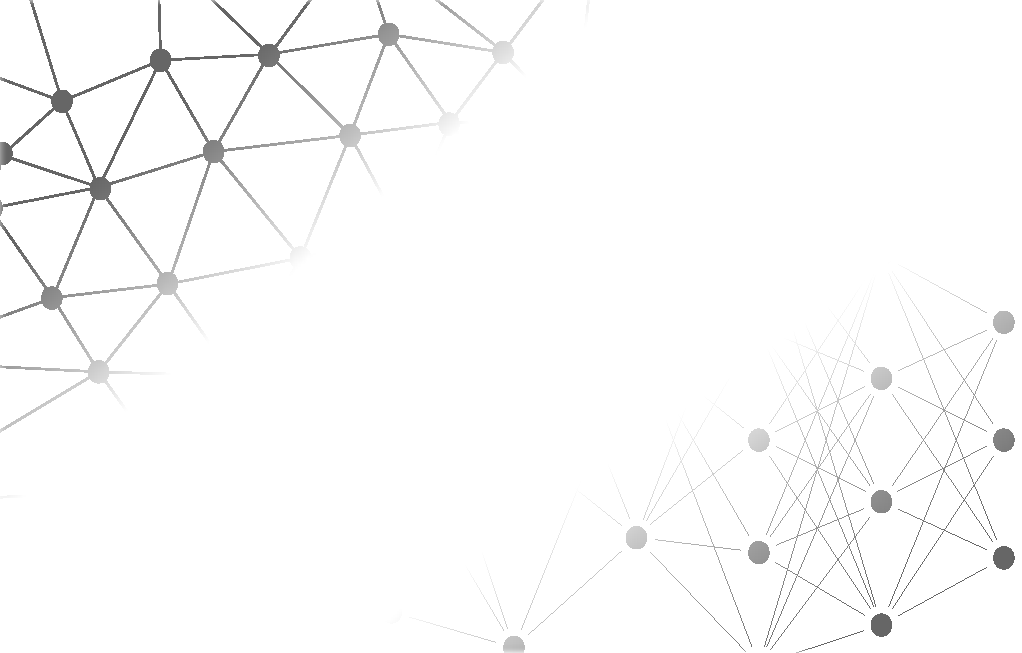
\includegraphics[width=\paperwidth,height=\paperheight]{Background.pdf}};
		\end{tikzpicture}
	}
	\begin{frame}[plain]
		\centering
		\begin{minipage}{0.21\textwidth}
			\centering
			
\includegraphics[width=\linewidth]{Bauhaus_Logo.png}
		\end{minipage}\hspace{105pt}
		\begin{minipage}{0.3\textwidth}
			\centering
			
\includegraphics[width=\linewidth]{JHU_Logo.png}
		\end{minipage}
		
		\titlepage
		\vspace{-35pt}
		Bauhaus Spring School 2026
		
	\end{frame}
}

%====================================================
\begin{frame}{Motivation}
  \centering
  \textbf{Why weak forms?}\\[1em]
  \begin{itemize}
    \item Physical equations (PDEs) are usually given in \textbf{strong form}.
    \item Strong forms require smooth solutions — often too restrictive.
    \item The \textbf{weak form} relaxes this requirement and is the starting point for FEM approximations.
  \end{itemize}
  \vfill
  \textit{In this part of the course, we use the Poisson equation as our running case study (for both FEM and later PINNs / Neural Operators)}
\end{frame}

%====================================================
\begin{frame}{The Strong Form - Possion Equation in 1D}
  
  \begin{block}{Poisson Equation}
  	\centering
  	\[
  	-\frac{d^2u}{dx^2} = f(x), \quad x\in(0,L),
  	\qquad u(0)=0,\; u(L)=0
  	\]
  	
  	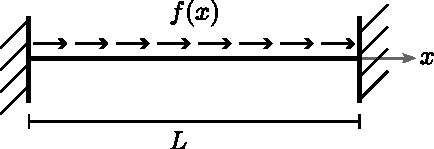
\includegraphics[width=0.5\linewidth]{Figures/Pure_Dirichlet_1D.pdf}
  \end{block}
  
  \vspace{0.5cm}

  \textbf{Requirements:} 
  \begin{itemize}
  	\item $u(x)$ must be twice differentiable
  	\item The equation holds pointwise
  \end{itemize}

  \vspace{0.3cm}
\end{frame}

%====================================================
\begin{frame}{From Strong to Weak Form}
  \footnotesize
  \textbf{General steps for obtaining the weak form:}
  \begin{enumerate}
  	\item Multiply by a test function ($v(x)$ with $v(0)=v(L)=0$) and integrate over $x\in (0,L)$:
  	\[
  	\int_0^L \! \big(-u''v\big)\,dx = \int_0^L f v\,dx
  	\]
  	
  	\item Integrate by parts:
  	\[
  	\int_0^L u'v'\,dx = \int_0^L f v\,dx
  	\]
  \end{enumerate}
  \textbf{Result:} Weak form reduces derivative order on $u$.

	\vspace{10pt}
	
	\hspace{20pt}
	\begin{minipage}{0.4\textwidth}
		\centering
		\textbf{Strong Form}
		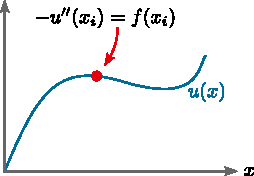
\includegraphics[width=0.8\linewidth]{Figures/Slide2_1.pdf}
		\textit{Pointwise Equilibium}
	\end{minipage}\hfill
	\begin{minipage}{0.4\textwidth}
		\centering
		\textbf{Weak Form}
		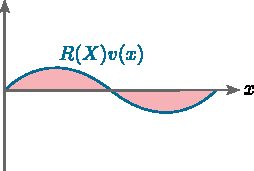
\includegraphics[width=0.85\linewidth]{Figures/Slide2_2.pdf}
		\textit{Weighted Average $=0$}
	\end{minipage}
	\hspace{20pt}

\end{frame}

%====================================================
\begin{frame}{Integration by Parts and Boundary Terms}
  \footnotesize
  Integrating $\int_0^L (-u''v)\,dx$ by parts:
  \[
  \int_0^L -u''v\,dx = [-u'v]_0^L + \int_0^L u'v'\,dx
  \]
  \vspace{0.3cm}
  For $v(0)=v(L)=0$ (Pure Dirichlet Problem):
  \[
  \int_0^L u'v'\,dx = \int_0^L f v\,dx
  \]
  For Neumann BC at $x=L$ ($u'(x=L)=g$):
  \[
  \int_0^L u'v'\,dx = \int_0^L f v\,dx + g v(L)
  \]

  \vfill
  
  \begin{itemize}
  	\item  \textit{Dirichlet BCs: imposed on the function space $\Rightarrow$ We only allow test functions that already satisfy $u=0$ at the Dirichlet boundary.}
  	\item \textit{Neumann BCs: appear naturally.}
  \end{itemize}
 
  	 
\end{frame}

%====================================================
\begin{frame}{Extension to 2D}
	\footnotesize
  \begin{minipage}{0.4\textwidth}
  	\centering
  	
  	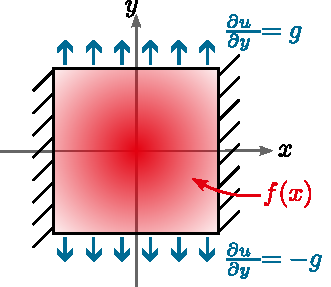
\includegraphics[width=\linewidth]{Figures/Poisson_2D.pdf}
  	
  \end{minipage}\hfill
  \begin{minipage}{0.56\textwidth}
  	\[
  	-\Delta u = f \quad \text{in } \Omega
  	\]
  	\[
  	u=0 \text{ on } \Gamma_D, \quad \nabla  u\cdot\mathbf{n}=g \text{ on } \Gamma_N
  	\]
  	\begin{align*}
  		\mbox{where } \;\Gamma_D &\Rightarrow \mbox{Dirichlet Boundary}\\
  		\Gamma_N &\Rightarrow \mbox{Neumann Boundary}
  	\end{align*}
  \end{minipage}
  
  \vfill
	\vspace{10pt}
  Integration by parts in 2D:
  \begin{equation*}
  	\int_\Omega -\Delta uvd\Omega = \int_\Omega \nabla u\cdot\nabla v d\Omega - \int_{\partial \Omega}(\nabla u\cdot \mathbf{n})v d\Gamma
  \end{equation*}
  If $v=0$ on $\Gamma_D$, and $\nabla  u\cdot\mathbf{n}=g$ on $\Gamma_N$:
  \[
  \int_\Omega \nabla u \cdot \nabla v\,d\Omega
  = \int_\Omega f v\,d\Omega + \int_{\Gamma_N} g v\,d\Gamma
  \]

\end{frame}

%====================================================
\begin{frame}{Example: Constant Load in 1D}
  \[
  -u''=1, \quad u(0)=u(L)=0
  \]
  Weak form:
  \[
  \int_0^L u'v'\,dx = \int_0^L v\,dx
  \]
  Exact solution:
  \[
  u(x)=\frac{x(L-x)}{2}
  \]

  \vfill
  \textit{The exact solution satisfies both strong and weak forms.}
\end{frame}

%====================================================
\begin{frame}{Strong vs Weak: Concept Summary}
  \centering
  \vspace{0.3cm}
  \footnotesize
  \begin{block}{Strong form}
  	\begin{itemize}
  		\item Equation type $\Rightarrow$ Differential (pointwise)
  		
  		\item Smoothness $\Rightarrow$ Twice differentiable ($C^2$)
  		
  		\item Boundary Conditions $\Rightarrow$ Dirichlet \& Neumann written explicitly in the equation
  		
  		\item FEM compatibility $\Rightarrow$ $\times$
  	\end{itemize}
  \end{block}

	
	\begin{block}{Weak form}
		\begin{itemize}
			\footnotesize
			\item Equation type $\Rightarrow$ Integral (averaged)
			
			\item Smoothness $\Rightarrow$ Needs only 1 derivative of 
			u (derivative square-integrable) ($H^1$)
			
			\item Boundary Conditions 
			\begin{itemize}
				\footnotesize
				\item Dirichlet built into admissible functions (trial/test space)
				\item Neumann appears automatically as boundary integrals
			\end{itemize}
			
			\item FEM compatibility $\Rightarrow$ $\checkmark$
		\end{itemize}
	\end{block}
  
\end{frame}

%====================================================
\begin{frame}{Closing Remarks}
  \begin{center}
  \Large
  \textit{Why strong vs weak forms matter beyond FEM}
  \end{center}

  \vspace{0.5cm}
  \small
  \begin{itemize}
  	\item FEM: discretize the weak form → element matrices via integrals.
  	\item PINNs: minimize a loss function, which is set in terms of either the strong or the weak form.
  	\item Neural Operators: often trained on data produced from weak-form discretizations.
  \end{itemize}

\end{frame}

%====================================================
\end{document}
